\emph{Convolutional networks}, also \emph{ConvNets} or \emph{CNNs}, were first inspired by the way the human visual cortex proccesses information~\cite{Fukushima1980} but, as regular neural networks, have evolved to favor practical performance over biological accuracy. LeCun et al. used a convolutional network to achieve good classification performance on the MNIST data set of handwritten digits~\cite{LeCun1989, LeCun1998}, the first successful application of modern convolutional networks. Recently, Krizhevsky et al. used  them to achieve state-of-the-art performance on the ImageNet Large-Scale Visual Recognition Challenge~\cite{Krizhevsky2012}, an image classification and object localization challenge with 1000 categories~\cite{Russakovsky2014}. Thanks to various advances (maxpooling, ReLU activations, weight initialization, GPU training, efficient backpropagation, etc.), convolutional networks have become one of the most popular methods for image classification tasks and (along with recursive neural networks) an emblem of deep learning.

In this section we show the standard features and training of current convolutional networks. Section~\ref{subsec:PracticalDL} gives some practical advice for choosing hyperparameters and training deep architectures. For an in depth review of convolutional networks, see \cite{Karpathy2015}. For a complete overview of the history and state of deep learning, see \cite{Schmidhuber2015}.

Convolutional networks map raw image pixels to a score vector $h_\Theta(x) \in \mathbb{R}^K$ representing the distribution of (unnormalized log) probabilities over the $K$ classes. We could use a regular neural network (presented in Section~\ref{subsec:ANNs}) to do this but the amount of learnable parameters (the weights) becomes very big. For instance, a small color image of size $100\times100$ with 3 color channels (RGB) will require $30\,000$ units in the input layer and each unit in the second layer will therefore have $30\,000$ weights to learn. This is impractical not only because it will require a lot of data and training time but because the loss function has very many local minima and thus it is harder to optimize.

Convolutional networks reduce the number of connections between layers and the number of parameters to learn. Convolutional layers are \emph{sparsely connected}, i.e., a unit is only connected to a small subset of the units in the previous layer. Furthermore, they are \emph{locally connected}, i.e., units are connected considering their position on the original image. The architecture of a convolutional network also imposes \emph{weight sharing} between units in the same layer, i.e., different units are forced to share the same weights (this determines filters and feature maps, defined below). \emph{Pooling} is a subsampling mechanism that reduces the spatial scale and makes the computations invariant to local translation. All these features reduce computation and improve the classification performance of convolutional networks; they are produced by the way convolutional networks are defined, which we explain below.

Each layer is composed of a set of \emph{feature maps}, 2-dimensional grids of unit activations~($\mathbb{R}^{h\times w}$), arranged into a 3-dimensional matrix ($\mathbb{R}^{h\times w \times d}$). We use the third dimension to put together all feature maps. One could unfold a 3-dimensional volume to form a single column of unit activations as in regular neural networks but seeing them as a volume makes the definitions easier. The input layer is a 3-dimensional matrix ($\mathbb{R}^{h\times w \times c}$) that holds the input image of size $w\times h$ with $c$ color channels ($c = 1$ for grayscale images or $c = 3$ for RGB). The output layer is a volume of size $R^{1\times 1 \times K}$ where each feature map is just one activation ($R^{1\times 1}$) representing the final score. The network receives an image $x$ as an input volume that is transformed layer by layer into new volumes (whose dimensions could be different from the previous one) until it reaches the output layer of size $h(x) = R^{1\times 1 \times K}$. See Fig.~\ref{fig:ConvNetVolumes} for an illustration. We describe the transformations next.
\begin{figure}[h]
	\centering
	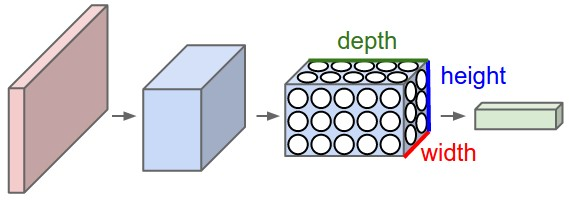
\includegraphics[width = 0.7\textwidth]{plots/convNetVolumes.jpeg}
	\caption[Convolutional network visualization]{A simple representation of the transformations of the input computed by a convolutional network. Input layer is shown in pink, hidden layers are shown in blue and output layer is shown in green. The third layer has 5 feature maps of size $2\times3$. Notice that the width is listed first by convention. Image courtesy of~\cite{Karpathy2015}.}
	\label{fig:ConvNetVolumes}
\end{figure}

Four types of layers are commonly used: convolutional layer, ReLU layer, pooling layer and fully connected layer; all of which compute a differentiable function on its input and combine to form a convolutional network architecture.

\paragraph{Convolutional layer} Convolutional layers are the heart of convolutional networks. They are build by learnable filters that are applied to the volume in the previous layer. A \emph{filter} is a matrix of weights that has a small spatial size (width and height) but goes across all feature maps of the volume (the third dimension). For instance, a $3\times 3$ filter to be applied in a volume with 10 feature maps will have 90 parameters ($\mathbb{R}^{3\times3\times10}$). See Figure~\ref{fig:ConvLayer} for an example. Each feature map in this layer is obtained by sliding a filter across the spatial dimensions (width and height) of the previous volume computing the dot product (a weighted sum) between the filter and the input~\footnote{Each filter has also a bias term added to the sum.}. All values in a single feature map are computed using the same filter. If we think of the feature map as a grid of units we can see that every unit is connected with only a small local subset of the units in the previous layer and that all units in the map share the same weights. 

At each convolutional layer, many feature maps are computed (each with its own filter) and stacked together to form the volume in the layer. We can think of each filter as looking for an specific feature on the input and each feature map as the probabilities of that feature in each position.

We choose various hyperparameters for this layer: the filter size, the stride (the number of places to shift the filter at each step), the amount of zero padding around the image and the number of feature maps. These define the shape of the resulting volume; the first three are usually chosen to preserve the spatial size of the previous volume, the number of feature maps depends on the amount of features we want to learn.
\begin{figure}[h]
	\centering
	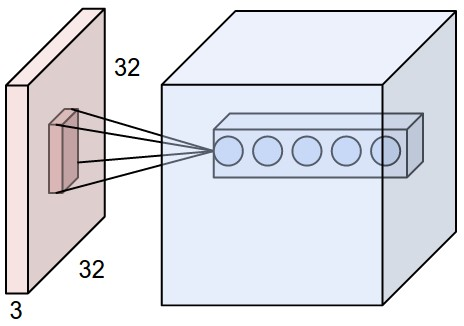
\includegraphics[width = 0.4\textwidth]{plots/convLayer.jpeg}
	\caption[Example of a filter in a convolutional layer]{Example of a filter applied to a volume ($\mathbb{R}^{32\times 32\times 3}$) to obtain the values shown in the blue volume. The filter comprises all 3 feature maps of the input volume. We compute 5 feature maps as shown by the 5 units in the blue volume. For a complete convolution this filter will have to slide across the input volume. All units in the same feature map share the same filter but units in different feature maps do not, even though they can be connected to the same local region of the input. Image courtesy of~\cite{Karpathy2015}.}
	\label{fig:ConvLayer}
\end{figure}

\paragraph{ReLU layer} This layer receives an input volume and performs an elementwise ReLU activation function to it, i.e, each value $z$ in the volume is passed through the nonlinearity $\max(0,z)$. It preserves the dimensions of the volume and has no learnable parameters, although the activation function may be considered a hyperparameter. Usually, a ReLU layer (or any other activation function) follows a convolutional layer, for this reason it is sometimes considered part of the convolutional layer. We separate them for clarity.

\paragraph{Pooling layer} The pooling layer subsamples the volume on the spatial dimensions reducing the size of the feature maps but keeping the number fixed. Standard max pooling slides a fixed size windows (normally $2\times2$) along each feature map with stride 2 (it is, without overlapping) and selects the maximum element on that space. This will reduce each dimension of the feature map by half, thus reducing the total number of activations by 75\%, e.g., a $4\times4$ feature map gets subsampled to size $2\times 2$ where each value is the maximum activation on each of the four quadrants of the original feature map. Contrary to convolution, subsampling is applied to each feature map separately. A popular variant of max pooling uses $3\times 3$ windows with stride 2, allowing for some overlapping.

\paragraph{Fully connected layer} We use one or more fully connected layers at the end of the network to compute the final score vector. Feature maps in this layer have size $1 \times 1$ resulting in a row volume or alternatively a row vector of values. Each feature map in this layer is fully connected to all units in the previous volume and outputs a dot product between the input and the connection weights, which are the parameters to be learned during training. The output layer of a convolutional network is always a fully connected layer with as many feature maps as classes. We interpret the scores of the output layer similar to those of regular neural networks as the (unnormalized log) probability of $x$ belonging to class $k$. Lastly, notice that a fully connected layer can be simulated by a convolutional layer with the same number of feature maps and filter size $w\times h$ where $w$ and $h$ are the spatial dimensions of the previos volume, i.e., filters that comprise the entire volume.

\bigskip
Convolutional layers (plus ReLUs) compute features on the input while pooling layers shrinken the volume before passing to the fully connected layers that act as a regular neural network classifier on the obtained features. The standard convolutional network architecture can be represented textually as:
\begin{verbatim}
       INPUT -> [[CONV -> RELU]*N -> POOL?]*M -> [FC -> RELU]*K -> FC
\end{verbatim}
where \texttt{*N} indicates that the layers are repeated \texttt{N} times, \texttt{?} indicates that the layer is optional and \texttt{N,M,K >= 0}. We can use this template to construct ever more flexible models from a linear classifier \texttt{INPUT -> FC} (\texttt{N,M,K = 0}) to a regular neural network \texttt{INPUT -> [FC -> RELU]+ -> FC} (\texttt{N,M = 0}, \texttt{K > 0}) to a convolutional network \texttt{INPUT -> [[CONV -> RELU]+ -> POOL?]+ -> [FC -> RELU]* -> FC} (\texttt{N,M > 0}, \texttt{K >= 0}). For instance, a typical deep convolutional network could be:
\begin{verbatim}
        INPUT -> [[CONV -> RELU]*2 -> POOL]*3 -> [FC -> RELU]*2 -> FC
\end{verbatim}
This network receives an input volume (the image) computes two sets of convolution plus ReLUs before pooling and repeats this pattern three times followed by fully connected layers plus ReLUs which are repeated twice and the output layer that reports the final classification scores. Although there is no standard way of counting the number of layers, we usually ignore the ReLU and pooling layers as they have no learnable parameters. Therefore, our example has 10 layers (21 in total), which is a good depth for big data sets. Practical recommendations on building architectures is offered in the Section~\ref{subsec:PracticalDL}.

Figure~\ref{fig:ConvNetExample} shows an example of a convolutional network with its different kind of layers. The image is taken from a simulation accesible at \url{cs231n.stanford.edu}.

\begin{figure}[h]
	\centering
	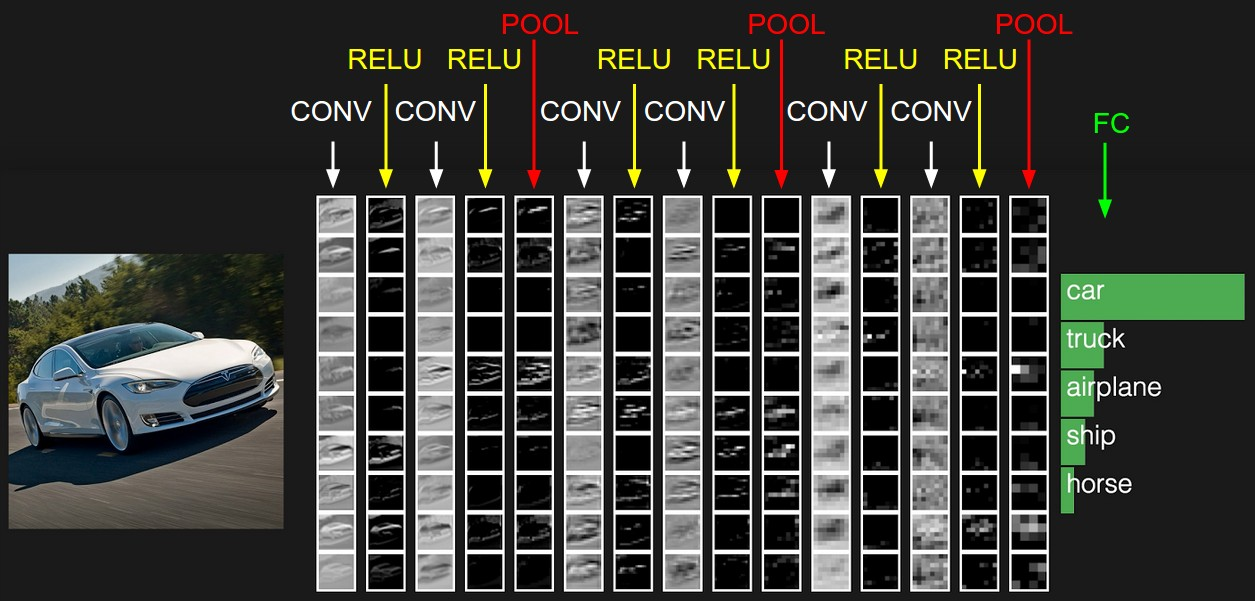
\includegraphics[width = 0.85\textwidth]{plots/convNetExample.jpeg}
	\caption[Example of a convolutional network in action]{Example of a convolutional network with architecture \texttt{INPUT -> [[CONV -> RELU]*2 -> POOL]*3 -> FC}. The input image has size $32\times 32$. Each hidden layer uses 10 feature maps (shown as columns). Although the spatial size of the feature maps looks constant in the image, each pooling layer reduces its dimensions by half (the feature maps of the final pooling layer have size $4\times 4$). We show the final scores only for the five most probable classes. Image courtesy of~\cite{Karpathy2015}.}
	\label{fig:ConvNetExample}
\end{figure}

Recently, simpler convolutional network architectures have emerged. The All Convolutional Net~\cite{Springenberg2014} is a network formed solely by convolutional layers: we replace pooling layers by convolutional layers with larger strides and fully connected layers as explained above. This greatly increases the number of parameters to be learn, therefore it is unsuitable for small data sets.

Converting the fully connected layers to convolutional layers has another advantage: we can use a convolutional network trained on small images to classify bigger images. By the way convolutional layers are defined when we use a bigger image as input the entire convolutional network will slide across the image and be applied to different portions of the image generating a score vector for each of them. Therefore, instead of having a single score for each class we will have an entire matrix of scores (for each position where the convolutional network was applied). Then, we can average over all scores per class to obtain a single score vector for the bigger image. Furthermore, we can control the stride of the convolution to choose how the convolutional network is slided across the big image.
For instance, if we train a convolutional network with images of size $32\times 32$ that via pooling get reduced to feature maps of size $4\times 4$ in turn passed to the (converted) fully connected layers to obtain a score vector, then when using a $96\times 96$ image as input to the same convolutional network it will get reduced to feature maps of size $12 \times 12$ and the fully connected layers will output a matrix of scores of size $9\times 9$ (for each class), i.e, it slides the $4\times 4$ fully connected layers across the $12\times 12$ feature maps. Averaging each score matrix we obtain the final scores for the big image. We could have also  set a stride of 4 in the first (converted) fully connected layer to get score matrices of size $3\times 3$ for each 9 non-overlapping $32\times 32$ partitions of the original image. It works exactly as if we applied the convolutional network to the original image at a stride of 32 but does all computations in just one pass. This way we can reuse a pretrained network to classify images of bigger size. 

\emph{Transfer learning} is a related method where we train a convolutional network on images from a specific domain and later use it to extract features on images from a different domain. It could also be used as a initialized network which is fine tuned with examples of the new domain.

The loss function for a multiclass convolutional neural network is similar to that for a regular neural network (Equation~\ref{eq:ANNRegularizedLossFunction}) except that now the convolutional network defines the vector score $h_\Theta(x)$.
\begin{equation}
	J(\Theta) = -\frac{1}{m} \sum_{i=1}^m \log \left ( \frac{ e^{h_\Theta(x^{(i)})_{y^{(i)}}} }{ \sum_{j=1}^K e^{ h_\Theta (x^{(i)})_j} } \right ) + \frac{\lambda}{2m}\sum_{l=1}^{L-1}\sum_{i=1}^{s^{(l)}}\sum_{j=1}^{s^{(l+1)}} \left(\Theta^{(l)}_{ij}\right)^2
	\label{eq:ConvNetLossFunction}
\end{equation}
Furthermore, this loss function is still differentiable with respect to $\Theta$ and thus we can train the entire network via gradient descent. We use backpropagation to calculate the gradients of the loss function.
